\begin{figure}
    \centering
    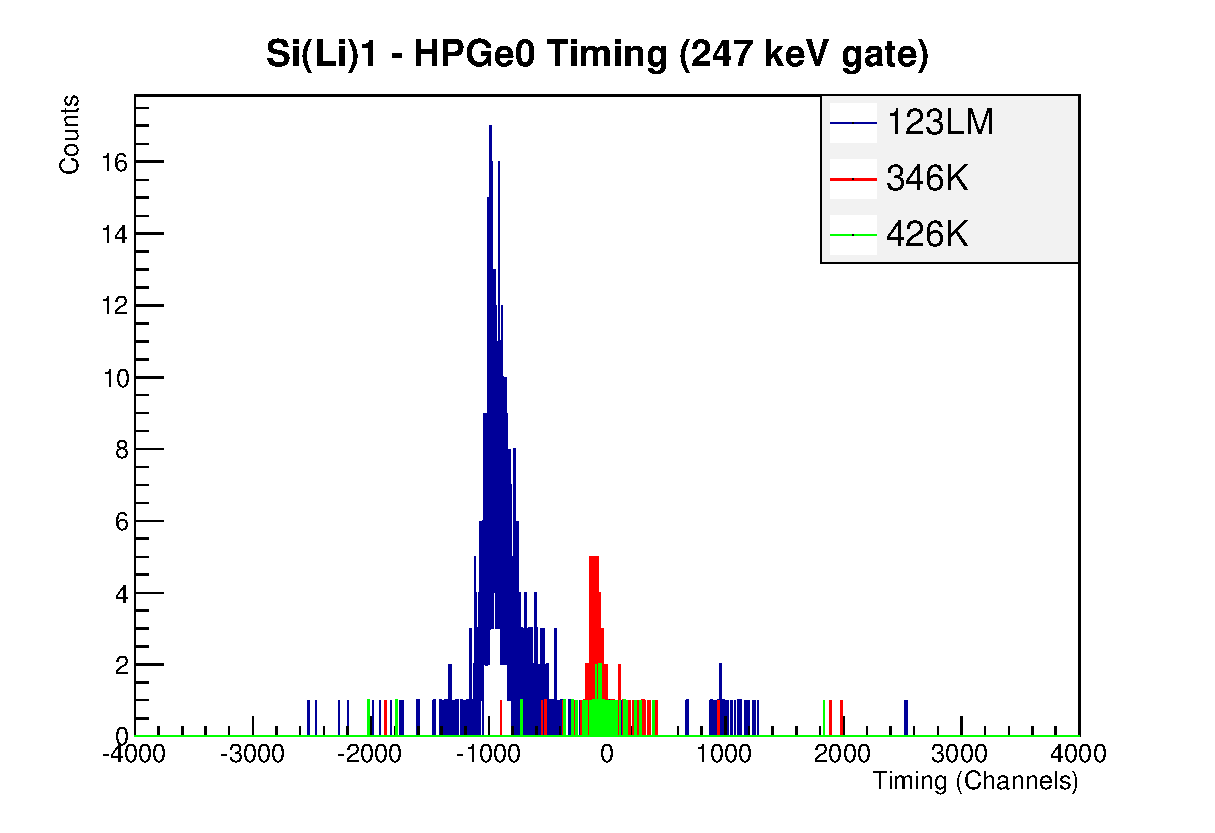
\includegraphics[scale=0.7]{Analysis_Figs/TimingvEnergy.eps}
    \caption{A plot of the energy-gated timing for a HPGe-Si(Li) detector pairing. The HPGe detector was gated at 247.9 keV, one of the ground state band transitions in the $^{145}$Gd nucleus. The conversion electrons for other transitions in the ground state band were gated on in the Si(Li) detector. Plotted here are the time differences between the two detectors when both peaks were seen in the respective detectors. The 123LM peak was used instead of the K peak due to the high threshold of this detector. As can be seen, the timing has an energy dependence. This dependence is most prominent at lower energies.}
    \label{fig:timing_georgina}
\end{figure}